% Options for packages loaded elsewhere
\PassOptionsToPackage{unicode}{hyperref}
\PassOptionsToPackage{hyphens}{url}
%
\documentclass[
]{book}
\usepackage{lmodern}
\usepackage{amssymb,amsmath}
\usepackage{ifxetex,ifluatex}
\ifnum 0\ifxetex 1\fi\ifluatex 1\fi=0 % if pdftex
  \usepackage[T1]{fontenc}
  \usepackage[utf8]{inputenc}
  \usepackage{textcomp} % provide euro and other symbols
\else % if luatex or xetex
  \usepackage{unicode-math}
  \defaultfontfeatures{Scale=MatchLowercase}
  \defaultfontfeatures[\rmfamily]{Ligatures=TeX,Scale=1}
\fi
% Use upquote if available, for straight quotes in verbatim environments
\IfFileExists{upquote.sty}{\usepackage{upquote}}{}
\IfFileExists{microtype.sty}{% use microtype if available
  \usepackage[]{microtype}
  \UseMicrotypeSet[protrusion]{basicmath} % disable protrusion for tt fonts
}{}
\makeatletter
\@ifundefined{KOMAClassName}{% if non-KOMA class
  \IfFileExists{parskip.sty}{%
    \usepackage{parskip}
  }{% else
    \setlength{\parindent}{0pt}
    \setlength{\parskip}{6pt plus 2pt minus 1pt}}
}{% if KOMA class
  \KOMAoptions{parskip=half}}
\makeatother
\usepackage{xcolor}
\IfFileExists{xurl.sty}{\usepackage{xurl}}{} % add URL line breaks if available
\IfFileExists{bookmark.sty}{\usepackage{bookmark}}{\usepackage{hyperref}}
\hypersetup{
  pdftitle={Magallanes Entrena: Reporte de resultados},
  pdfauthor={Matías Castillo},
  hidelinks,
  pdfcreator={LaTeX via pandoc}}
\urlstyle{same} % disable monospaced font for URLs
\usepackage{longtable,booktabs}
% Correct order of tables after \paragraph or \subparagraph
\usepackage{etoolbox}
\makeatletter
\patchcmd\longtable{\par}{\if@noskipsec\mbox{}\fi\par}{}{}
\makeatother
% Allow footnotes in longtable head/foot
\IfFileExists{footnotehyper.sty}{\usepackage{footnotehyper}}{\usepackage{footnote}}
\makesavenoteenv{longtable}
\usepackage{graphicx,grffile}
\makeatletter
\def\maxwidth{\ifdim\Gin@nat@width>\linewidth\linewidth\else\Gin@nat@width\fi}
\def\maxheight{\ifdim\Gin@nat@height>\textheight\textheight\else\Gin@nat@height\fi}
\makeatother
% Scale images if necessary, so that they will not overflow the page
% margins by default, and it is still possible to overwrite the defaults
% using explicit options in \includegraphics[width, height, ...]{}
\setkeys{Gin}{width=\maxwidth,height=\maxheight,keepaspectratio}
% Set default figure placement to htbp
\makeatletter
\def\fps@figure{htbp}
\makeatother
\setlength{\emergencystretch}{3em} % prevent overfull lines
\providecommand{\tightlist}{%
  \setlength{\itemsep}{0pt}\setlength{\parskip}{0pt}}
\setcounter{secnumdepth}{5}
\usepackage{booktabs}
\usepackage[]{natbib}
\bibliographystyle{apalike}

\title{Magallanes Entrena:
Reporte de resultados}
\author{Matías Castillo}
\date{2021-01-04}

\begin{document}
\maketitle

{
\setcounter{tocdepth}{1}
\tableofcontents
}
\hypertarget{introducciuxf3n}{%
\chapter{Introducción}\label{introducciuxf3n}}

La obesidad y el sobrepeso son factores determinantes a la hora de evaluar el riesgo de múltiples condiciones de salud, algunas de ellas como la diabetes, hipertensión, patología coronaria, accidentes cardiovasculares o cerebrovasculares, siendo que muchas de estas figuran como parte de los mayores problemas de la salud, tanto en el ámbito personal como en el impacto que esto tiene en el gasto público en salud y en políticas públicas orientadas a combatir la creciente epidemia de personas con obesidad.

El sedentarismo, junto con la obesidad, representan a la actualidad uno de los mayores factores de riesgo para la salud y, han sido asociados a un aumento en la complicaciones orgánicas a múltiples niveles en el cuerpo humano. Pese a lo anterior, el cambio en los estilos de vida ha sido propuesto por diversos especialistas como una estrategia de bajo costo para tratar de revertir el riesgo que estas condiciones representan para la salud de las personas y para el gasto público actual.

El ejercicio físico ha mostrado ser eficaz para mejorar marcadores de riesgo cardiovascular en adultos obesos/as, junto con reducir el riesgo de mortalidad por cualquier causa. Sumado a lo anterior, el asesoramiento en materia de nutrición y adopción de estilos de vida saludables ha mostrado ser capaz de generar una mayor adherencia a programas de ejercicio físico a diferencia del entrenamiento sin asesoramiento alguno.

Por esto, el equipo de \href{https://www.australfitness.cl}{Austral Fitness ®} organizó una serie de actividades de promoción de estilos de vida saludables mediante el uso de ejercicio grupal supervisado y charlas de nutrición, todo esto bajo el financiamiento del Fondo de Fortalecimiento de la Secretaría General de Gobierno.

\hypertarget{metodos}{%
\chapter{Material y métodos}\label{metodos}}

\hypertarget{sujetos}{%
\section{Sujetos}\label{sujetos}}

Para el proyecto y su consecución, la implementación de formularios fue clave para la inscripción de los participantes, así como el seguimiento de los mismos. Del mismo modo, se les aplicó el cuestionario SF-36 para evaluar parámetros de salud y calidad de vida, en conjunto con un cuestionario de actividad física (i.e.~IPAQ)

De los sujetos evaluados (n = 217), el 79\% de quienes respondieron las encuestas fueron de la Región de Magallanes. Del total de la muestra, la proporción de cada región puede apreciarse en la Tabla \ref{tab:regiones}.

\label{tab:regiones} Proporción de personas por sexo en cada región.

\begin{tabular}{l|l|l|l}
\hline
**Characteristic** & Hombre & Mujer & **Total**\\
\hline
\_\_Región\_\_ &  &  & \\
\hline
Región de Antofagasta & 0\% & 0.5\% & 0.5\%\\
\hline
Región de Aysén del General Carlos Ibáñez del Campo & 2.3\% & 7.4\% & 9.7\%\\
\hline
Región de Coquimbo & 0\% & 0.5\% & 0.5\%\\
\hline
Región de La Araucanía & 0\% & 0.5\% & 0.5\%\\
\hline
Región de Los Lagos & 0\% & 0.9\% & 0.9\%\\
\hline
Región de Los Ríos & 0\% & 0.5\% & 0.5\%\\
\hline
Región de Magallanes y la Antártica Chilena & 16\% & 63\% & 79\%\\
\hline
Región de Valparaiso & 0.5\% & 2.8\% & 3.2\%\\
\hline
Región del Biobío & 0\% & 0.5\% & 0.5\%\\
\hline
Región del Libertador General Bernardo O´Higgins & 0\% & 0.9\% & 0.9\%\\
\hline
Región del Maule & 0\% & 0.5\% & 0.5\%\\
\hline
Región Metropolitana & 0\% & 3.7\% & 3.7\%\\
\hline
\_\_Total\_\_ & 18\% & 82\% & 100\%\\
\hline
\end{tabular}

\hypertarget{sf-36}{%
\section{SF-36}\label{sf-36}}

El SF-36 Health Survey es una encuesta de salud diseñada por el Health Institute, New England Medical Center, de Boston Massachusetts, que a partir de 36 preguntas pretende medir ocho conceptos genéricos sobre la salud, esto es, conceptos que no son específicos de una patología, grupo de tratamiento o edad, detectando tanto estados positivos como negativos de la salud física y estado emocional.

Los ocho conceptos de salud (dimensiones) determinados en este cuestionario se resumen en la tabla \ref{tab:sf36-table}.

\begin{table}

\caption{\label{tab:sf36-table}Dominios evaluativos en el cuestionario SF-36.}
\centering
\begin{tabular}[t]{ll}
\toprule
Dimensión & Significado\\
\midrule
Función física & Grado en el que la falta de salud limita las actividades físicas de la vida diaria, como el cuidado personal, caminar, subir escaleras, coger o transportar cargas, y realizar esfuerzos moderados e intensos.\\
Rol físico & Grado en el que la falta de salud interfiere en el trabajo y otras actividades diarias, produciendo como consecuencia un rendimiento menor del deseado, o limitando el tipo de actividades que se puede realizar o la dificultad de las mismas.\\
Dolor corporal & Medida de la intensidad del dolor padecido y su efecto en el trabajo habitual y en las actividades del hogar.\\
Salud general & Valoración personal del estado de salud, que incluye la situación actual y las perspectivas futuras y la resistencia a enfermar.\\
Vitalidad & Sentimiento de energía y vitalidad, frente al de cansancio y desánimo.\\
\addlinespace
Función social & Grado en el que los problemas físicos o emocionales derivados de la falta de salud interfieren en la vida social habitual.\\
Rol emocional & Grado en el que los problemas emocionales afectan al trabajo y otras actividades diarias, considerando la reducción del tiempo dedicado, disminución del rendimiento y del esmero en el trabajo\\
Salud mental & Valoración de la salud mental general, considerando la depresión, ansiedad, autocontrol, y bienestar general.\\
\bottomrule
\end{tabular}
\end{table}

\hypertarget{ipaq}{%
\section{IPAQ}\label{ipaq}}

La actividad física fue evaluada mediante el Cuestionario Internacional de Actividad Física (IPAQ), que es una herramienta de medición de uso común. Diseñado como un cuestionario estandarizado de autoinforme, el IPAQ puede proporcionar a los investigadores y profesionales una estimación de la actividad física y el comportamiento sedentario de los adultos de 15 a 69 años de edad, en una variedad de entornos socioeconómicos. Además, el IPAQ también es beneficioso para los investigadores que colaboran dentro de un mismo país o entre países en diferentes lugares. En la actualidad, el IPAQ se explora en relación con su capacidad para medir el comportamiento sedentario.

Los parámetros de asociación entre categorías de actividad física y sexo no muestran una relación entre si, sin embargo, la proporción de mujeres es significativamente mayor en cada categoría de actividad física, lo que puede ser evidenciado en la Figura \ref{fig:sexo-vs-actfisc}.

\begin{figure}

{\centering 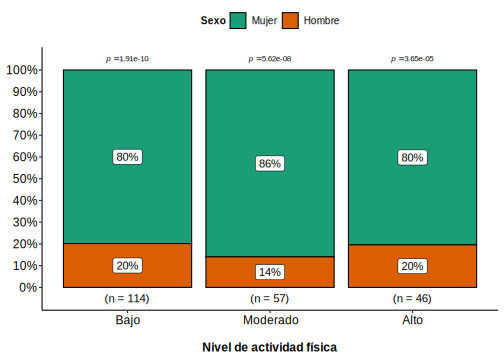
\includegraphics[width=1\linewidth]{reportes_files/figure-latex/sexo-vs-actfisc-1} 

}

\caption{Proporción de hombres y mujeres en cada nivel de actividad física en toda la muestra}\label{fig:sexo-vs-actfisc}
\end{figure}

\hypertarget{entrenamiento-computarizado}{%
\section{Entrenamiento computarizado}\label{entrenamiento-computarizado}}

El periodo de entrenamiento consistió en 5 clases computarizadas de acondicionamiento físico a la semana por un periodo de 12 semanas supervisado por un entrenador en cada clase, en el cual se realizaron ejercicios de musculación de intensidad moderada (i.e.~OMNI-RES 5-6/10) en una estructura de entrenamiento tipo circuitos para inducir un aumento del gasto cardíaco en el ejercicio y la solicitación de sistemas energéticos aeróbicos y anaeróbicos lácticos.

\hypertarget{talleres-de-nutriciuxf3n}{%
\section{Talleres de nutrición}\label{talleres-de-nutriciuxf3n}}

De forma complementaria se realizaron talleres de nutrición orientados a la adopción y mantenimiento de estilos de alimentación saludables junto con brindar estrategias nutricionales para favorecer su adherencia en combinación con programas de ejercicio físico. Éstas actividades fueron realizadas vía conferencia virtual al igual que los entrenamientos computarizados.

\hypertarget{anuxe1lisis-estaduxedstico}{%
\section{Análisis estadístico}\label{anuxe1lisis-estaduxedstico}}

Para el análisis estadístico se consideraró a los sujetos correspondientes a la Región de Magallanes como la unidad de análisis sobre la cual se realizarán estadísticos descriptivos, correlacionales y contrastes de hipótesis sobre parámetros de tendencia central.

El software de programación para la computación estadística R \citep{R-base} en su versión 4.0.3 fue utilizado para los análisis implementados en este reporte. Para la significación estadística se fijó un \(\alpha\) igual al 5\%. Para las pruebas de contraste de hipótesis de la tendencia central de los grupos a evaluar se utilizó la prueba Wilcoxon-Mann-Whitney, esto debido a violaciones de la normalidad en los contrastes de categorías con dos niveles y, la prueba Kruskall-Wallis para las comparaciones de categorías con 3 niveles. Para las pruebas de asociación entre variables categóricas se utilizó la prueba \(\chi{}^2\) de Pearson.

Como unidad de medida de tamaño de efecto (ES) se utilizó la \(d\) de Cohen para las comparaciones de grupos mediante la prueba \(t\) de Student; \(\eta{}^2\) como ES para ANOVA y la \(V\) de Cramer para la prueba de \(\chi{}^2\) de Pearson.

\hypertarget{resultados}{%
\chapter{Resultados}\label{resultados}}

\hypertarget{actividad-fuxedsica}{%
\section{Actividad física}\label{actividad-fuxedsica}}

De la muestra evaluada perteneciente a la Región de Magallanes (n = 171), el 19.9\% (n = 34) correspondió a hombres y el 80.1\% (n = 137) a mujeres. La edad de los evaluados fue de 32 ± 9 años, sin diferencias entre hombres y mujeres (\(log_e({W}_{Mann-Whitney})\) = 7.76, \(p\) = 0.988, \(\widehat{r}\) = 0.00).

\begin{figure}
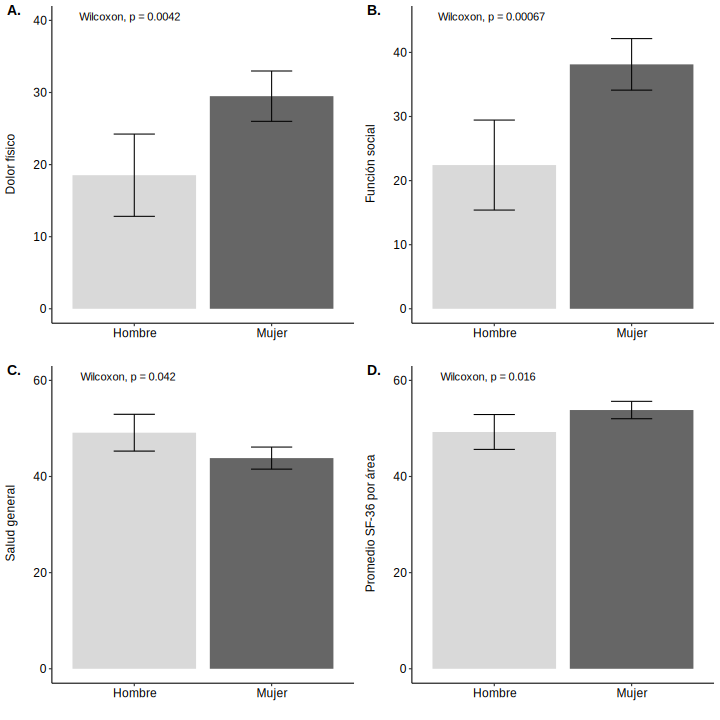
\includegraphics[width=1\linewidth]{reportes_files/figure-latex/sf36-plots-1} \caption{Parámetros del SF-36 ajustados por sexo.}\label{fig:sf36-plots}
\end{figure}

En parámetros de actividad física, pudimos evaluar la distribución de los índices de los equivalentes metabólicos (MET's) relacionados con el gasto energético y en consecuencia a la actividad física asociada, el cual fue obtenido de manera indirecta mediante el cuestionario IPAQ, en donde observamos una leve tendencia en los hombres a tener un mayor gasto energético total por semana (1,508 ± 2,162 MET's/semana) en comparación con las mujeres (1,141 ± 1,374 MET's/semana), sin embargo estas diferencias no fueron estadísticamente significativas (\(log_e({W}_{Mann-Whitney})\) = 7.80, \(p\) = 0.657, \(\widehat{r}\) = 0.03). En relación a la clasificación de actividad física, el 53\% de los sujetos fueron catalogados con un nivel bajo de actividad física, un 25\% con un nivel medio y un 22\% con un nivel alto (Tabla \ref{tab:summary-sexo}), sumado a lo anterior se destaca que no hubo un patrón que indicara una asociación entre la clasificación de actividad física y el sexo (\(\chi^2_{~Pearson}\)(2) = 1.38, \(p\) = 0.502, \(V_{~Cramer's}\) = 0.09).

\label{tab:summary-sexo} Valores por variable de estudio para los grupos de cada nivel de la categoría sexo de la submuestra correspondiente a la Región de Magallanes.

\begin{tabular}{l|l|l|l|l}
\hline
**Variables** & **Total** & **Hombre**, N = 34 & **Mujer**, N = 137 & **P-valor**\\
\hline
\_\_Edad\_\_ & 32 ± 9 & 32 ± 10 & 32 ± 9 & 0.986\\
\hline
\_\_MET's /semana\_\_ & 1,214 ± 1,562 & 1,508 ± 2,162 & 1,141 ± 1,374 & 0.656\\
\hline
\_\_Actividad física\_\_ &  &  &  & 0.502\\
\hline
Bajo & 90 (53\%) & 19 (56\%) & 71 (52\%) & \\
\hline
Moderado & 43 (25\%) & 6 (18\%) & 37 (27\%) & \\
\hline
Alto & 38 (22\%) & 9 (26\%) & 29 (21\%) & \\
\hline
\_\_Dolor corporal\_\_ & 27 ± 20 & 19 ± 16 & 29 ± 21 & \_\_0.004\_\_\\
\hline
\_\_Función física\_\_ & 90 ± 17 & 92 ± 14 & 89 ± 17 & 0.337\\
\hline
\_\_Función social\_\_ & 35 ± 24 & 22 ± 20 & 38 ± 24 & \_\_<0.001\_\_\\
\hline
\_\_Rol emocional\_\_ & 80 ± 36 & 73 ± 41 & 82 ± 35 & 0.160\\
\hline
\_\_Rol físico\_\_ & 62 ± 43 & 59 ± 45 & 63 ± 43 & 0.570\\
\hline
\_\_Salud general\_\_ & 45 ± 13 & 49 ± 11 & 44 ± 14 & \_\_0.042\_\_\\
\hline
\_\_Salud mental\_\_ & 41 ± 9 & 38 ± 11 & 41 ± 8 & 0.057\\
\hline
\_\_Vitalidad\_\_ & 44 ± 10 & 43 ± 11 & 44 ± 10 & 0.816\\
\hline
\_\_Evolución de salud\_\_ &  &  &  & 0.698\\
\hline
Peor & 13 (7.6\%) & 4 (12\%) & 9 (6.6\%) & \\
\hline
Algo peor & 59 (35\%) & 9 (26\%) & 50 (36\%) & \\
\hline
Igual & 53 (31\%) & 11 (32\%) & 42 (31\%) & \\
\hline
Algo mejor & 24 (14\%) & 5 (15\%) & 19 (14\%) & \\
\hline
Mucho mejor & 22 (13\%) & 5 (15\%) & 17 (12\%) & \\
\hline
\_\_SF-36 Score\_\_ & 53 ± 11 & 49 ± 10 & 54 ± 11 & \_\_0.016\_\_\\
\hline
\end{tabular}

\hypertarget{salud-seguxfan-sf-36}{%
\section{Salud según SF-36}\label{salud-seguxfan-sf-36}}

En relación a lo obtenido en el cuestionario SF-36, podemos destacar el componente de dolor corporal, el cual representa una ``\emph{Medida de la intensidad del dolor padecido y su efecto en el trabajo habitual y en las actividades del hogar}'' en el que las mujeres tuvieron una puntuación significativamente mayor en comparación a los hombres (\(log_e({W}_{Mann-Whitney})\) = 7.38, \(p\) = 0.004, \(\widehat{r}\) = -0.22), sin embargo al ajustar por el nivel de actividad física no encontramos diferencias estadísticamente significativas entre los niveles de esta categoría (\(\chi_{~Kruskall-Wallis}^2\)(2) = 2.03, \(p\) = 0.363, \(\epsilon^2\) = 0.01). En relación a la función social, evaluada dentro del SF-36, las mujeres puntuaron (38 ± 24) más que los hombres (22 ± 20), \(log_e({W}_{Mann-Whitney})\) = 7.29, \(p\) = 0.001, \(\widehat{r}\) = -0.26, pero al igual que con el parámetro de dolor físico, al ajustar la función social según la condición física de los participantes no encontramos diferencias significativas entre los participantes (\(\chi_{~Kruskall-Wallis}^2\)(2) = 0.08, \(p\) = 0.963, \(\epsilon^2\) = 0.00).

\begin{figure}
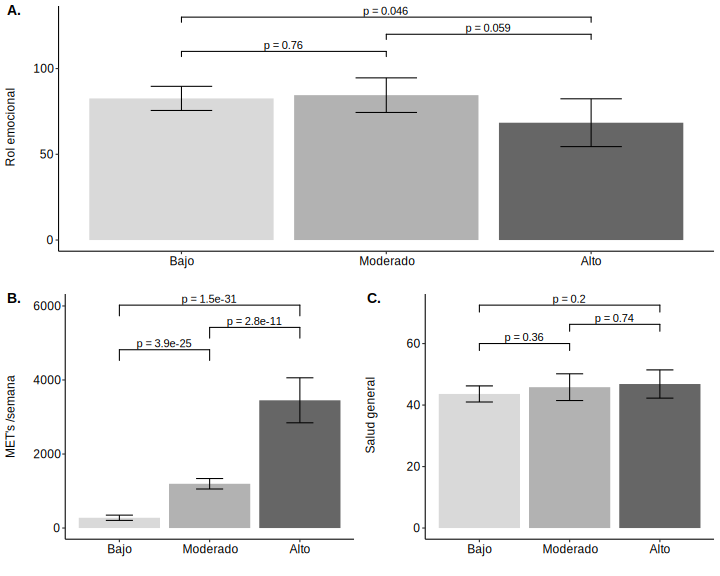
\includegraphics[width=1\linewidth]{reportes_files/figure-latex/sf36-plots2-1} \caption{Parámetros del SF-36 ajustados por nivel de actividad física.}\label{fig:sf36-plots2}
\end{figure}

Respecto al parámetro de salud general, el cual se define como ``\emph{Valoración personal del estado de salud, que incluye la situación actual y las perspectivas futuras y la resistencia a enfermar}'', los datos muestran que en promedio, los hombres (49 ± 11) puntúan mejor que las mujeres (44 ± 14), \(log_e({W}_{Mann-Whitney})\) = 7.96, \(p\) = 0.042, \(\widehat{r}\) = 0.16, sin embargo, y al ajustar por parámetros de actividad física no se hallaron diferencias significativas en los rangos medios de los grupos de actividad física (\(\chi_{~Kruskall-Wallis}^2\)(2) = 3.85, \(p\) = 0.146, \(\epsilon^2\) = 0.02). Los detalles en relación a los grupos se muestran en la Tabla \ref{tab:summary-sexo} y \ref{tab:summary-actfisc}.

\label{tab:summary-actfisc} Valores por variable de estudio para los grupos de cada nivel de la categoría actividad física de la submuestra correspondiente a la Región de Magallanes.

\begin{tabular}{l|l|l|l|l}
\hline
**Variables** & **Bajo**, N = 90 & **Moderado**, N = 43 & **Alto**, N = 38 & **P-valor**\\
\hline
\_\_Edad\_\_ & 32 ± 9 & 31 ± 9 & 33 ± 9 & 0.648\\
\hline
\_\_Sexo\_\_ &  &  &  & 0.502\\
\hline
Hombre & 19/90 (21\%) & 6/43 (14\%) & 9/38 (24\%) & \\
\hline
Mujer & 71/90 (79\%) & 37/43 (86\%) & 29/38 (76\%) & \\
\hline
\_\_MET's /semana\_\_ & 278 ± 341 & 1,196 ± 460 & 3,451 ± 1,848 & \_\_<0.001\_\_\\
\hline
\_\_Dolor corporal\_\_ & 29 ± 18 & 27 ± 22 & 25 ± 23 & 0.363\\
\hline
\_\_Función física\_\_ & 90 ± 14 & 92 ± 14 & 87 ± 24 & 0.059\\
\hline
\_\_Función social\_\_ & 35 ± 24 & 36 ± 25 & 35 ± 24 & 0.963\\
\hline
\_\_Rol emocional\_\_ & 83 ± 34 & 84 ± 33 & 68 ± 42 & 0.087\\
\hline
\_\_Rol físico\_\_ & 61 ± 44 & 69 ± 43 & 59 ± 41 & 0.468\\
\hline
\_\_Salud general\_\_ & 44 ± 12 & 46 ± 14 & 47 ± 14 & 0.146\\
\hline
\_\_Salud mental\_\_ & 41 ± 10 & 39 ± 7 & 42 ± 9 & 0.135\\
\hline
\_\_Vitalidad\_\_ & 44 ± 11 & 43 ± 9 & 46 ± 9 & 0.388\\
\hline
\_\_Evolución de salud\_\_ &  &  &  & \\
\hline
Peor & 11/90 (12\%) & 1/43 (2.3\%) & 1/38 (2.6\%) & \\
\hline
Algo peor & 33/90 (37\%) & 18/43 (42\%) & 8/38 (21\%) & \\
\hline
Igual & 30/90 (33\%) & 12/43 (28\%) & 11/38 (29\%) & \\
\hline
Algo mejor & 10/90 (11\%) & 7/43 (16\%) & 7/38 (18\%) & \\
\hline
Mucho mejor & 6/90 (6.7\%) & 5/43 (12\%) & 11/38 (29\%) & \\
\hline
\_\_SF-36 Score\_\_ & 53 ± 10 & 54 ± 10 & 51 ± 13 & 0.667\\
\hline
\end{tabular}

  \bibliography{book.bib,packages.bib}

\end{document}
